\section{Sesión 4}

\begin{teorema}
	Una función monótona $f:[a,b]\to\mathbb{R}$ es Riemann-integrable. 
\end{teorema}

\begin{nota}
	Una función monótona no es necesariamente continua [¿Qué sucede si $f$ tiene un conjunto no contable de discontinuidades de salto en $[a,b]$?]
\end{nota}

\begin{prop}
	Sea 
	$$\int_a^b c f=c\int_a^b f\qquad (f\in R[a,b]).$$
\end{prop}


\begin{nota}
	Sean $f$ y $g$ funciones acotadas sobre el intervalo $I\implies f+g$ es acotada. 
\end{nota}

\begin{prop}(Supremos e ínfimos)
	$$\sup_I (f+g)\leq \sup_I(f)+\sup_I (g)$$
	$$\inf_I (f+g)\geq \inf_I(f)+\inf_I (g)$$
\end{prop}

\begin{prop} Sea
	$$\operatorname{osc}_I (f+g)=\operatorname{osc}_I (f)+\operatorname{osc}_I (g)$$
\end{prop}

\begin{prop}
	$f,g\in R(I)\implies f+g\in R(I)$. 
\end{prop}

\begin{nota}
	Las integrales superior e inferior de funciones no integrables no son, en general, lineales.
\end{nota}


\begin{definicion}
	Sea $a<b$. 
	\begin{enumerate}
		\item $\overline{\int_a^b}f:=-\overline{\int_a^b}f$ y $\underline{\int_a^b} f :=-\underline{\int_b^a}f$. Si las integrales coinciden, entonces: 
		$$\int_a^b f=-\int_b^a f.$$
		\item $\forall c\in [a,b]$, se define: $\overline{\int_c^c}f=\underline{\int_a^c}f=0.$
	\end{enumerate}
\end{definicion}

\begin{prop}(Varios)
	\begin{enumerate}
		\item $\overline{\int_a^b}(f+g)\leq \overline{\int_a^b}f+\overline{\int_a^b}g$. 
		\item $\underline{\int_a^b}(f+g)\leq \overline{\int_a^b}f+\underline{\int_a^b}g$. 
	\end{enumerate}
\end{prop}

\begin{teorema}
	Si $f,g\in R\implies \int_a^b(f+g)=\int_a^b f+\int_a^b g$. 
\end{teorema}

\begin{prop}(Monotonicidad)
	Sean $f,g\in R[a,b]$ y suponga que $f(x)\leq g(x),\forall x\in [a,b]$. Entonces: 
	$$\int_a^b f\leq \int_a^b f$$
\end{prop}


\begin{teorema}
	Suponga que $f\in R[a,b]$ y sea $M=\sup_{[a,b]}(f)$ y $m=\inf_{[a,b]}f$. Entonces, 
	$$m(b-a)\leq \int_a^b f\leq M(b-a).$$
\end{teorema}


\begin{teorema}(Valor medio para integrales)
	Si $f:[a,b]\to\mathbb{R}$ es continua, entonces $\exists c\in [a,b]\ni$ 
	
	$$f(c)=\frac{1}{b-a}\int_a^b f.$$
\end{teorema}
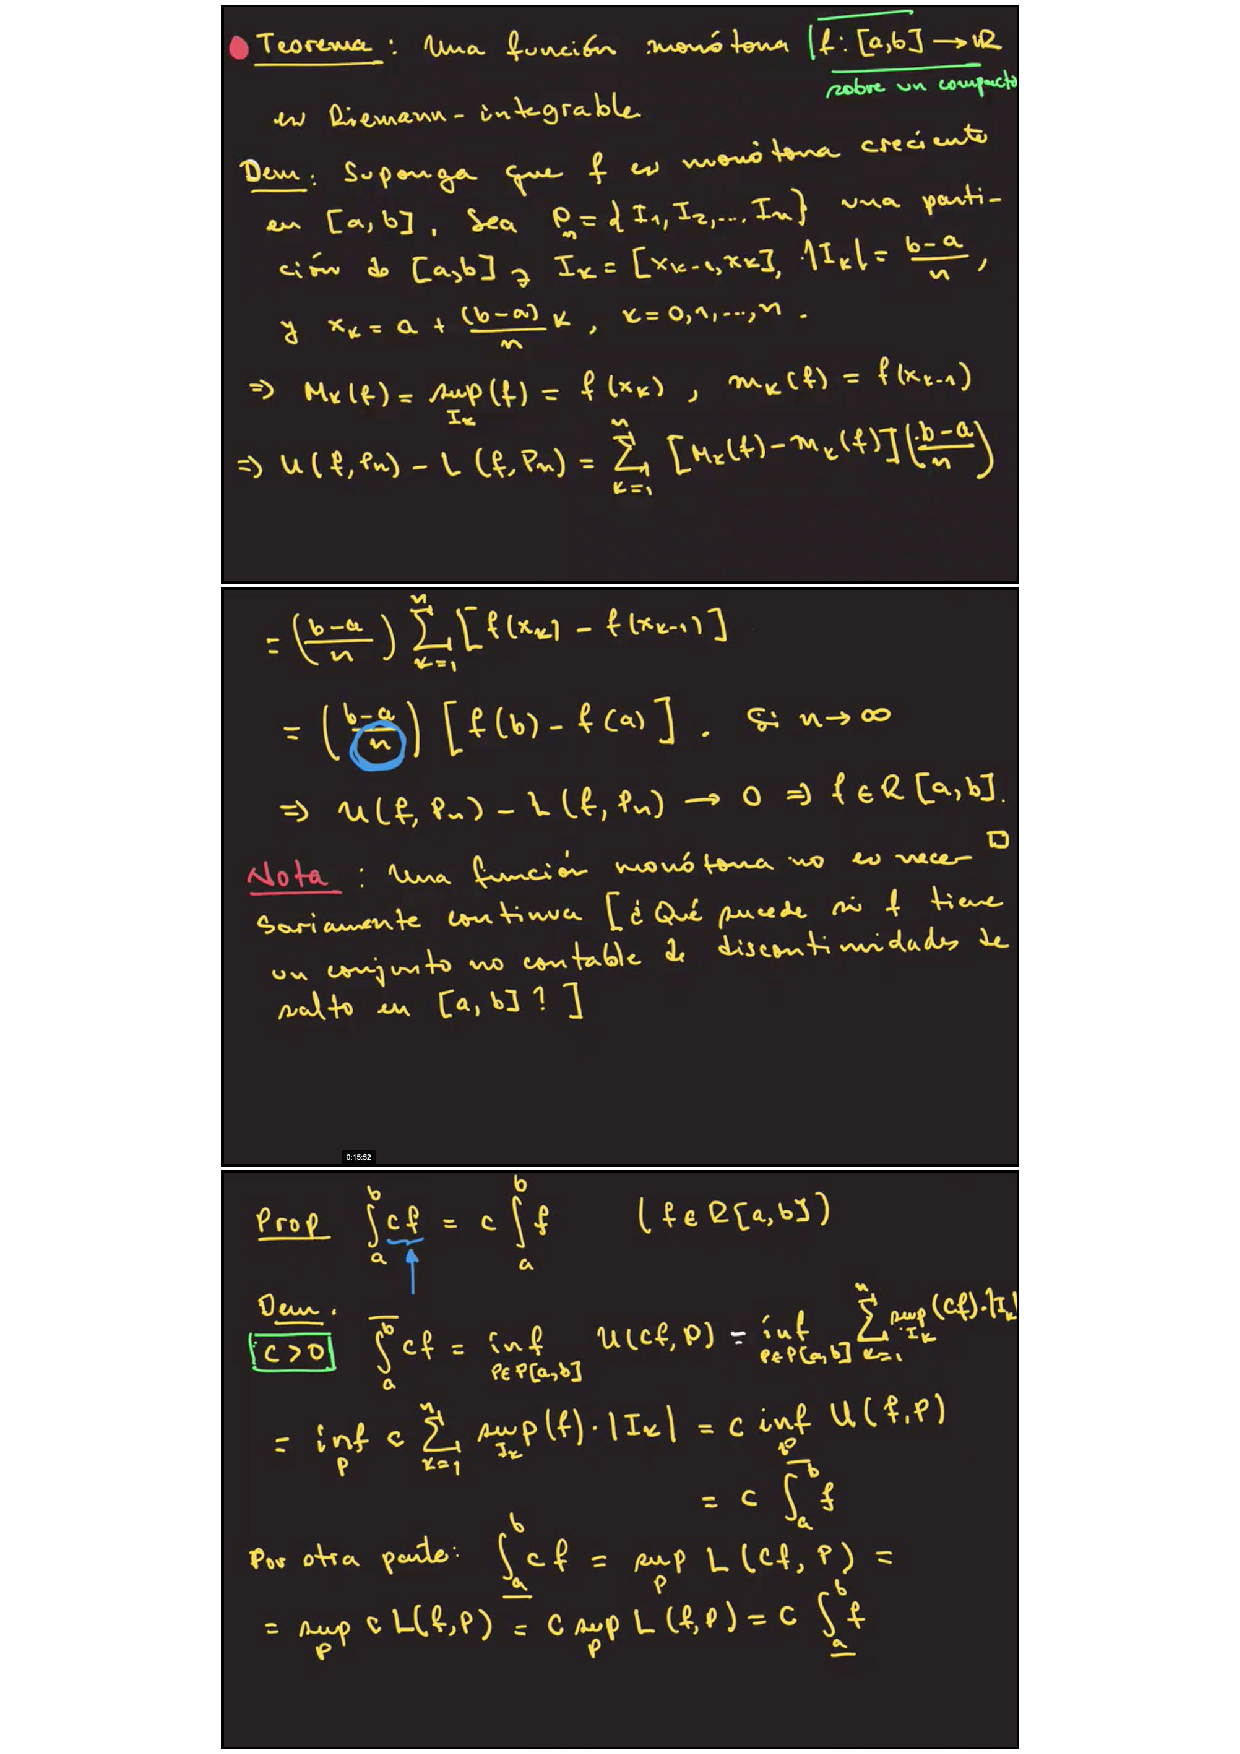
\includepdf[pages=-]{apendices/s4.pdf}